In the computer vision field, there has been increasing interest in object category recognition. Among the major tasks, image classification is defined as the task of assigning an image one or multiple labels corresponding to the presence of a category in the image.\\
Multi-label image classification is however a more
general and practical problem, since the majority of real-world images are with more than one objects
of different categories. Many methods
have been proposed to address this more challenging
problem. The success of CNN on single-label image
classification also sheds some light on the multi-label image classification problem. However, the CNN
model cannot be trivially extended to cope with the
multi-label image classification problem in an interpretable manner, mainly due to the following reasons.
Firstly, the implicit assumption that foreground objects are roughly aligned, which is usually true for
single-label images, does not always hold for multi-label images. Such alignment facilitates the design of
the convolution and pooling infrastructure of CNN
for single-label image classification. However, for a
typical multi-label image, different categories of objects are located at various positions with different
scales and poses. For example, as shown in Figure \ref{fig1},
for single-label images, the foreground objects are
roughly aligned, while for multi-label images, even
with the same label, i.e., cat and bird, the spatial arrangements of the cat and bird instances
vary largely among different images. Secondly, the
interaction between different objects in multi-label
images, like partial visibility and occlusion, also poses
a great challenge. Therefore, directly applying the
original CNN structure for multi-label image classification is not feasible. Thirdly, due to the tremendous
parameters to be learned for CNN, a large number of
training images are required for the model training.
Furthermore, from single-label to multi-label (with n
category labels) image classification, the label space
has been expanded from n to 2n, thus more training data is required to cover the whole label space. For
single-label images, it is practically easy to collect
and annotate the images. However, the burden of
collection and annotation for a large scale multi-label
image dataset is generally extremely high.\\
So we propose a simple technique using our trained single-label classifier of CNN with the objectness measure \cite{1} and selective search \cite{2}. First we segment a multi-label image into some segments or image windows using the two approaches and then test these images against our trained single label model and predict the multiple labels of the image. We have taken different approaches like taking top-1, top-2, total sum of the scores and cumulative percentage sum of the scores to predict the labels.

\begin{figure} 
    \centering
  \subfloat[a]{%
       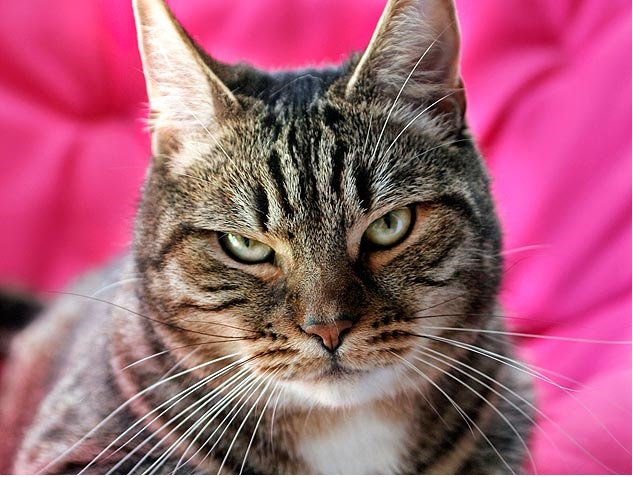
\includegraphics[width=0.2\linewidth]{images/1a}}
    \label{1a}
  \subfloat[b]{%
        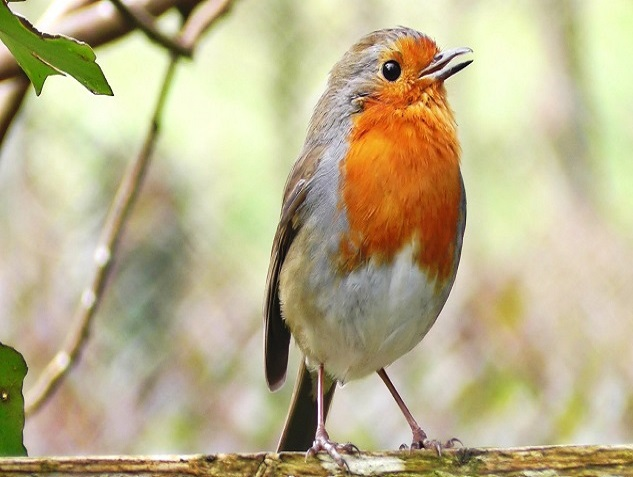
\includegraphics[width=0.2\linewidth]{images/1b}}
    \label{1b}
  \subfloat[c]{%
        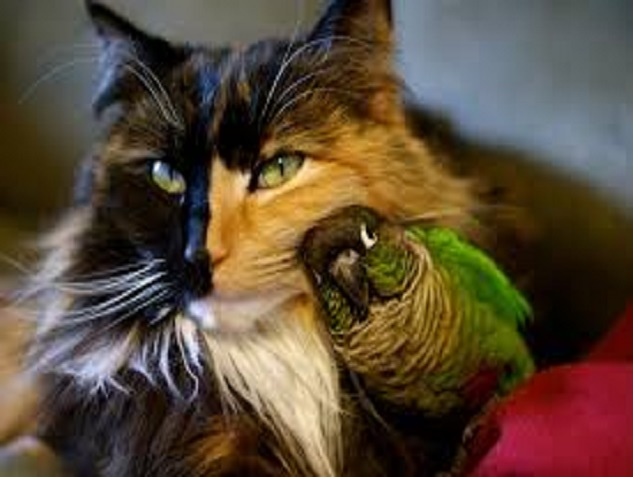
\includegraphics[width=0.2\linewidth]{images/1c}}
    \label{1c}
  \subfloat[d]{%
        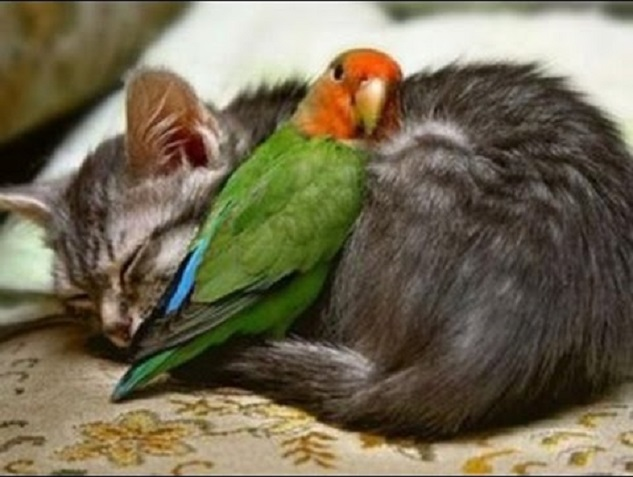
\includegraphics[width=0.2\linewidth]{images/1d}}
     \label{1d} 
  \caption{(a), (b) Some examples from CIFAR-10 \cite{4}. The objects in     
        single-label images are usually roughly aligned.(c),(d) However, the 
        assumption of object alignment is not valid for multi-label
        images. Also note the partial visibility and occlusion
        between objects in the multi-label images.}
        \vspace{-.5cm}
  \label{fig1} 
\end{figure}



%\newcolumntype{C}{>{\centering\arraybackslash}X} % centered version of "X" type
%\setlength{\extrarowheight}{1pt} % filler text
%\begin{table*}
% \caption{CIFAR-10 Confusion Matrix}
%\label{my-label}
%\begin{tabularx}{\textwidth}{@{}l*{10}{C}c@{}}
%\toprule
%labels     & airplane & automobile & bird & cat & deer & dog & frog & horse & ship & truck & accuracy \\ 
%\midrule
%airplane   & 915      & 4          & 17   & 19  & 3    & 1   & 0    & 2     & 27   & 12    & 91.50\%  \\ 
%automobile & 8        & 934        & 3    & 4   & 0    & 0   & 3    & 0     & 10   & 38    & 93.40\%  \\ 
%bird       & 60       & 1          & 813  & 37  & 19   & 23  & 30   & 10    & 7    & 0     & 81.30\%  \\ 
%cat        & 18       & 1          & 34   & 746 & 25   & 113 & 37   & 18    & 8    & 0     & 74.60\%  \\ 
%deer       & 24       & 1          & 38   & 33  & 809  & 19  & 44   & 29    & 2    & 1     & 80.90\%  \\ 
%dog        & 4        & 0          & 37   & 106 & 23   & 792 & 9    & 26    & 2    & 1     & 79.20\%  \\ 
%frog       & 2        & 5          & 19   & 35  & 1    & 20  & 912  & 2     & 3    & 1     & 91.20\%  \\ 
%horse      & 14       & 0          & 26   & 20  & 18   & 28  & 4    & 886   & 3    & 1     & 88.60\%  \\ 
%ship       & 35       & 10         & 3    & 2   & 0    & 2   & 1    & 0     & 936  & 11    & 93.60\%  \\ 
%truck      & 23       & 37         & 4    & 10  & 1    & 2   & 2    & 0     & 15   & 906   & 90.60\%  \\ 
%\bottomrule
%\end{tabularx}
%\end{table*}
